\enteteExam{NFP 107 -- Systèmes de gestion de bases de données - Durée 2h30}%
{Examen seconde session 31 août 2022}%
{Examen sur table -- Seuls documents autorisés\,: 10 pages maximum de notes manuscrites.}%

M. Hardy se prépare à déménager, ce qui nécessite
de ranger toutes ses affaires dans des cartons.
Afin de faciliter l'emménagement, il décide de constituer
une base de données pour savoir ce que contient
exactement chaque carton. Il donne donc un code
et un libellé à tous ses objets, un numéro à
tous ses cartons, et numérote également
les pièces de son ancien et de son nouvel appartement.

Ensuite, il indique, pendant l'emballage, dans quel
carton se trouve chaque objet. Un carton
contient les objets d'une même pièce d'origine, et
ces objets vont dans une même pièce de destination.
Il espère gagner beaucoup de temps grâce à cette base de données\,!

M. Hardy prend conseil auprès d'un de ses amis, M. Laurel, qui
crée alors un schéma relationnel avec les tables suivantes
(les clés étrangères ne sont pas représentées)\,:

      \begin{itemize}
        \item Pièce (\textbf{noPièce}, libellé, surface)
        \item Carton (\textbf{noCarton}, jourEmballage, noPièceOrigine,
                            noPièceDestination)
        \item  Objet (\textbf{codeObjet}, intitulé, poids,
                     noCarton)
       \end{itemize}

L'attribut \textit{jourEmballage} est l'un
des jours de la semaine (lundi, mardi, ...). Le libellé
de la pièce est quelque chose comme ``chambre'', ``salon'',
etc. La surface est exprimée en m$^2$.

\section{Schéma (6 pts)}

\begin{enumerate}

   \item ({\bf 1 pt}) Donnez les commandes {\tt create table} décrivant
         le schéma des relations ci-dessus. Indiquez soigneusement
         les clés étrangères et les clés primaires.


\begin{solution}
\begin{minted}{sql}
create table Pièce
   (noPièce integer not null,
    libellé varchar not null,
    surface integer not null,
     primary key(noPièce));

create table Carton
   (noCarton integer not null,
    jourEmballage varchar not null,
    noPièceOrigine integer not null,
    noPièceDestination integer not null,
     primary key(noCarton),
     foreign key (noPièceOrigine) references Pièce (noPièce),
     foreign key (noPièceDestination) references Pièce (noPièce));

create table Objet
   (codeObjet integer not null,
    intitulé varchar not null,
    poids integer not null,
    noCarton integer not null,
    primary key(codeObjet),
    foreign key (noCarton) references Carton (noCarton));
\end{minted}
\end{solution}

   \item ({\bf 1 pt}) Le schéma permet-il que la pièce d'origine soit la même
      que la pièce de destination\,? Si vous pensez que c'est le
      cas donnez la contrainte SQL qui
       force la pièce d'origine d'un carton à être
         différente de la pièce de destination.

\begin{solution}
Ajout de la contrainte SQL dans la table \texttt{Carton}:
\begin{minted}{sql}
check (noPièceOrigine != noPièceDestination)
\end{minted}
\end{solution}



  \begin{figure}[htb]
  \begin{center}
   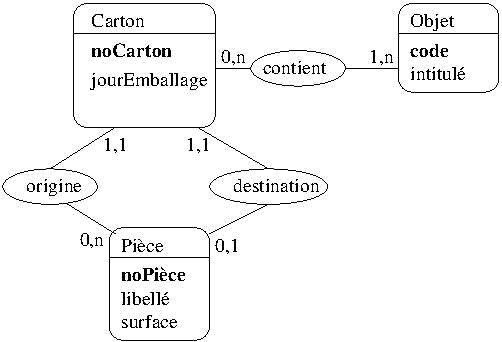
\includegraphics{../figures/schema-demenagement}
    \caption{Modélisation de la base du déménagement}
    \label{schema-hardy}
    \end{center}
  \end{figure}


    \item ({\bf 2 pts}) M. Hardy avait essayé de décrire son besoin avec le
      schéma entité-association de la figure~\ref{schema-hardy}.
     Ce schéma comporte des erreurs qui ont été corrigées
       par M. Laurel
       au moment de la création du schéma relationnel. Quelles
       sont ces erreurs\,?

\begin{solution}
Une pièce peut être la destination de plusieurs
cartons. Et les cardinalités sont inversées entre Pièce et Carton.
De même un
objet est contenu dans un seul carton.
\end{solution}

 \item ({\bf 1 pt}) Après de nouvelles discussions entre les deux amis, M. Laurel
        propose à M. Hardy une évolution du schéma pour prendre en compte
        des besoins plus complexes que ceux estimés à l'origine. Voici
        la nouvelle version \emph{proposée}.

      \begin{itemize}
        \item Pièce (\textbf{noPièce}, libellé, surface)
        \item Carton (\textbf{noCarton}, jourEmballage, noPièceOrigine)
        \item  Objet (\textbf{codeObjet}, intitulé, catégorie,
                     noCarton)
        \item Destination (\textbf{noCarton, idPièce})
       \end{itemize}
  À votre avis qu'est-ce qui peut motiver ce changement\,? Que pouvons-nous
 représenter maintenant qui n'était pas possible auparavant\,?

\begin{solution}
 Les objets d'un même carton peuvent maintenant être distribués dans plusieurs pièces.
\end{solution}


 \item ({\bf 1 pt}) À quoi correspondrait cette table \texttt{Destination} sur le schéma
 EA\,?

\begin{solution}
Association plusieurs à plusieurs entre \texttt{Carton} et \texttt{Pièce}.
\end{solution}
\end{enumerate}

\section{Requêtes (7 pts)}

Aidez M. Hardy à organiser son déménagement en
exprimant (en SQL) les requêtes suivantes. \textbf{Important}\,: ces requêtes sont à exprimer
sur le schéma donné dans l'énoncé, pas sur le schéma modifié proposé par M. Laurel.

\begin{enumerate}
% 1 pt
  \item Donnez l'intitulé de chaque objet, et le libellé de la pièce
    dont il provient.

% 1 pt
  \item Pour chaque carton emballé le jeudi, donnez le no du carton et les libellé et surface
      de la pièce d'origine et de la pièce de destination.
% 1 pts
  \item Quelles pièces sont l'origine d'un carton et la destination d'un autre carton\,?
% 1 pts
  \item Quelles pièces ne recevront aucun carton\,?
% 1 pts
  \item Donnez les pièces d'origine dont aucun carton n'a pour destination le salon.
% 1 pts
  \item Pour chaque carton indiquez le numéro du carton, le nombre d'objets et le poids du carton.
% 2 pts
  \item Pour chaque pièce recevant plus de 20 cartons, indiquez le libellé de la pièce, le
    nombre de cartons et le poids total.
  \end{enumerate}


\begin{solution}
Pièce (\textbf{noPièce}, libellé, surface)

Carton (\textbf{noCarton}, jourEmballage, noPièceOrigine,
                            noPièceDestination)

Objet (\textbf{codeObjet}, intitulé, poids,
                     noCarton)

\begin{minted}{sql}
select o.intitulé, p.libellé
from Pièce as p, Objet as o, Carton as c
where o.noCarton = c.noCarton
and p.noPièce = c.noPièceOrigine

select c.noCarton, p1.libellé as libelléOrig, p1.surface as surfOrig,
         p2.libellé as libelléDest, p2.surface as surfDest
from Pièce as p1, Pièce as p2, Carton as c
where c.noPièceOrigine = p1.noPièce
and c.noPièceDestination = p2.noPièce
and c.jourEmballage = 'jeudi'

select p.libellé
from Pièce as p, Carton as c1, Carton as c2
where c1.noPièceOrigine = p.noPièce
and c2.noPièceDestination = p.noPièce
and c1.noCarton != c2.noCarton

select p.libellé
from Pièce as p
where not exists (select * from Carton as c
                  where c.noPièceDestination = p.noPièce)

select p.libellé
from Pièce as p
where not exists (select * from Carton as c, Pièce as p2
                  where c.noPièceOrigine = p.noPièce
                  and   c.noPièceDestination = p2.noPièce
                  and p2.libellé = 'salon')

select c.noCarton, count(*) as nbObjets, sum(poids) as totalPoids
from Carton as c, Objet as o
where c.noCarton = o.noCarton
group by c.noCarton

select p.libellé, count(distinct c.noCarton) as nbCartons, sum(o.poids) as poidsTotal
from Pièce as p, Carton as c, Objet as o
where c.noPièceDestination = p.noPièce
and c.noCarton = o.noCarton
group by p.noPièce, p.libellé
having count(*) >= 20
\end{minted}
\end{solution}


\section{Algèbre relationnelle ({\bf 2 pts})}

Exprimez les requêtes 1 et 4 précédentes
en algèbre relationnelle.


\section{Equivalences logiques ({\bf 2 pts})}

Réécrire la requête suivante sans négation et sans disjonction logique
(mais l'inégalité \texttt{!=} est perrmise).


\begin{minted}{sql}
select p.libellé
from Pièce as p, Carton as c
where not (p.noPièce = c.noPièceOrigine or p.noPièce = c.noPièceDestination)
\end{minted}

Peut-on dire que cette requête sélectionne les pièces qui ne sont ni origine, ni destination
d'un carton\,?

\begin{solution}

\begin{minted}{sql}
select p.libellé
from Pièce as p, Carton as c
where p.noPièce != c.noPièceOrigine and p.noPièce != c.noPièceDestination
\end{minted}

On trouve les pièces pour les lesquelles il existe au moins un carton
qui n'a la pièce ni pour origine ni pour destination.
\end{solution}


\section{Modèle relationnel ({\bf 3 pts})}

Soit les attributs TGVER avec les dépendances fonctionnelles suivantes\,:
$TG \to E$; $R \to G$; $E \to G$.

\begin{enumerate}
  \item Quelle est la clé\,?
  \item Quel est le résultat de l'algorithme de normalisation\,?
  \item Ce résultat est-il en troisième forme normale\,?
\end{enumerate}


\begin{solution}
Tous les attriuts qui n'apparaissent pas à droite sont nécessairement
dans la clé, donc T, V  et R. On vérifie aisément que TVR est une clé
(la seule).

On a donc les relations (TGE), (RG) et (EG), auxquelles il faut ajouter la clé
(TVR). Le résultat est en troisième forme normale.

\end{solution}
